\chapter{Project Functions}
\label{vl:tc-project}

\dword{tc} works with consortia through the \dword{tb} to identify and
resolve technical issues.  As defined in the \dword{dune} Management
Plan (DMP), \dword{dune} \dword{tb} generates technical solutions and
recommends technical decisions to the \dword{dune} collaboration
\dword{exb}, which comprises all consortia scientific and technical
leads. The board meets regularly (approximately monthly) to review and
resolve technical issues with detector construction. It reports
through the \dword{exb} to collaboration management. The \dword{dune}
\dword{tb} is chaired by the \dword{dune} \dword{tcoord}. The
\dword{tc} engineering team meets regularly (approximately weekly) to
discuss detailed technical issues.  \Dword{tc} is not responsible for
financial issues, which are referred to the \dword{exb} and
\dword{rcoord}.

\Dword{tc} has several major project support tasks:
\begin{itemize}
\item Ensure that each consortium has a well defined and complete
  scope, that interactions between the consortia are sufficiently well
  defined, and that any remaining scope is covered by \dword{tc}
  through \dword{comfund} or flagged as missing scope to the
  \dword{exb} and \dword{rcoord}. In other words, ensure that the full
  detector scope is identified. Monitor interactions and consortia
  progress in delivering their scope.
\item Develop an overall project \dlong{ims}
  that includes reasonable production schedules, testing plans and a
  well developed installation schedule from each consortium. Monitor
  the \dword{ims} as well as individual consortium schedules.
\item Ensure that appropriate engineering and safety standards are
  developed, understood and agreed to by all key stakeholders and that these
  standards are conveyed to and understood by each
  consortium. Monitor the design and engineering work.
\item Ensure that all \dword{dune} requirements on \dword{lbnf} for
  conventional facilities, cryostat and cryogenics are clearly
  defined and understood by each consortium. Negotiate scope
  boundaries with \dword{lbnf}. Monitor \dword{lbnf} progress on
  final conventional facility, cryostat and cryogenics
  design and implementation.
\item Ensure that technical issues associated with scaling from
  \dword{protodune} have sufficient resources to enable the detector to be fully integrated and
  installed (converging on
  decisions made by the consortia).
\item Ensure that each consortium has fully developed and reviewed
  integration plans, \dword{qc} processes, requirements for
  the \dword{itf} and installation plans..
\end{itemize}

\Dword{tc} is responsible for technical quality and the schedule but
not for consortia funding or budgets.  \Dword{tc} will try to resolve
any issues it can but will likely push all financial issues to the
\dword{tb}, \dword{exb} and \dword{rcoord} for resolution.

\Dword{tc} maintains a web
page\footnote{\url{https://web.fnal.gov/collaboration/DUNE/DUNE\%20Project/\_layouts/15/start.aspx\#/}.}
with links to project documents. \Dword{tc} also maintains
repositories of project documents and drawings. These include the
\dword{wbs}, schedule, risk register, requirements, milestones,
strategy, detector models and drawings that define the \dword{dune}
detector.

\section{\dword{dune} Project Description}

The following sections describe the systems that track the progress of
the \dword{dune} project as well as the ways in which this large,
distributed organization is managed.

The \dword{dune} project builds on significant development in previous
large \dword{lartpc} detectors (ICARUS and MicroBooNE) and on
substantial development from LBNE and LBNO. One of the most important
elements that has significantly advanced the project development is
the successfully construction and operation of the \dword{protodune}
detectors. These detectors use full-size \dword{dune} components and
processes. The construction of \dword{protodune} has established
teams, production lines, QA and QC processes, installation, operation
and performance of the final \dword{dune} detectors. Based on the
success of \dword{protodune}, \dword{dune} has reached advanced technical
maturity, approaching (80\%). The designs have significantly advanced
from \dword{protodune} to \dword{dune}. Most subsystems completed
\dword{pdr} or 60\% reviews on design modifications beyond
\dword{protodune} in advance of the \dword{tdr}. The overall level of
design maturity is now $\sim$90\%. The breakdown of the design maturity
level for \dword{dsp} by subsystem is provided in
Table~\ref{tab:designmaturity}. The table shows the final \dword{dune}
design maturity at the time of \dword{protodune} and now at the time
of the \dword{tdr}, along with the estimated design effort or weight
of each subsystem. The \dword{apa} conceptual design was developed in
2010 and prototyped at 40\% scale and again in the 35-ton detector. The version
deployed in \dword{pdsp} is close to that for \dword{dsp} (85\%). The
cold electronics low noise system design, including feedthroughs,
cables and grounding, was successfully prototyped at large scale in
MicroBooNE and \dword{pdsp} and is 90\% mature. The front end chip has
gone through eight iterations and was successfully demonstrated in
MicroBooNE and \dword{pdsp} (90\%). The frontend motherboard has gone
through a similar number of iterations and was successfully
demonstrated in \dword{pdsp} (80\%). The ADC chip has evolved from a
previous version used in CMOS 180~nm technology that was tested to $-50\circ$C. (50\%). Key
elements of the COLDATA chip have been prototyped (25\%). The HV
design has evolved from ICARUS, MicroBooNE and the 35-ton detector.  It
has been prototyped in subsequent runs of the 35-ton detector and
demonstrated in \dword{pdsp} (80\%). The photon system ARAPUCA design
has been prototyped at small scale and in \dword{pdsp} (20\%). The
mechanical design has been extensively developed using the 35-ton
detector and \dword{pdsp} (85\%). The DAQ artdaq backend has been
developed in several experiments, including the 35-ton detector and
\dword{pdsp}. The DAQ FELIX frontend has been developed by ATLAS and
prototyped in \dword{pdsp}.
\begin{dunetable}
  [\dword{dsp} design maturity]
  {|p{0.1\linewidth}|rp{0.1\linewidth}|rp{0.25\linewidth}|rp{0.2\linewidth}|}
  {tab:designmaturity}
  {\dword{dsp} design maturity}
  System & Weight & \dword{protodune} & \dword{dune}   \\ \toprowrule
  DSS & 10\% & 75\% &  85\% \\ \colhline
  APA & 30\% & 85\% &  95\% \\ \colhline
  CE  & 20\% & 80\% &  90\% \\ \colhline
  PDS & 10\% & 50\% &  65\% \\ \colhline
  HVS & 15\% & 80\% &  95\% \\ \colhline
  DAQ & 10\% & 60\% &  80\% \\ \colhline
  CISC & 5\% & 80\% &  90\% \\ \colhline \colhline
  Total& 100\% & 76\% & 90\% \\ \colhline
\end{dunetable}

The design maturity of the \dword{ddp} detector is also quite
advanced. It builds on working noble liquid \dwords{tpc} for dark
matter and neutrinoless double beta decay experiments. A significant
benchmark is the operation of the $3\times1\times1$ demonstrator at
CERN. A critical test will be the operation of \dword{pddp} at CERN. A
similar table of design maturity for \dword{ddp} will be included
here.

%%%%%%%%%%%%%%%%%%%%%%%%%%%%%%%%
\section{Work Breakdown Stgructure (WBS)}
\label{sec:fdsp-coord-wbs}

The \dword{dune} \dword{wbs} has six categories at level 1 as shown in
Table~\ref{fig:WBS_level2}.  
\begin{dunefigure}[\dword{dune} \dword{wbs} at level 2]{fig:WBS_level2}
  {High level \dword{dune} \dword{wbs} to level 2.}
  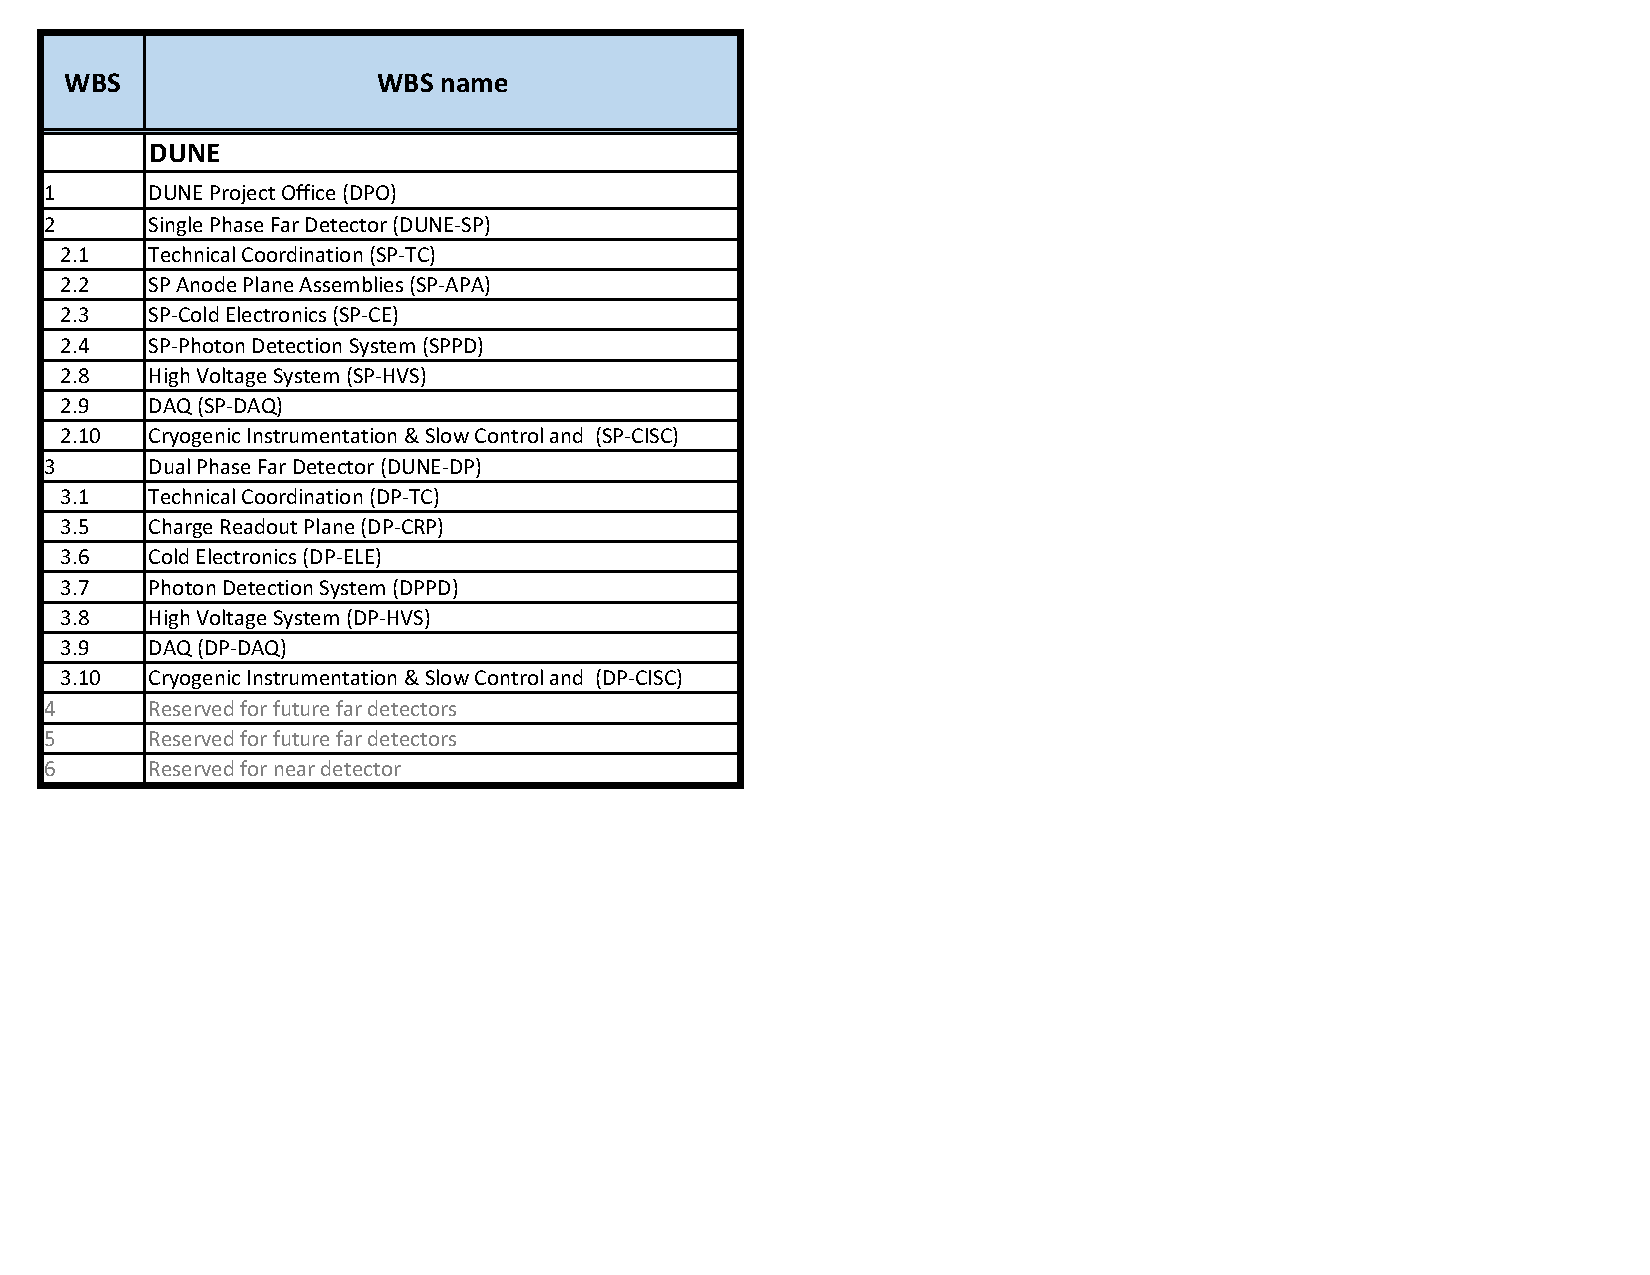
\includegraphics[width=0.75\textwidth]{WBS_level2}
\end{dunefigure}
At level 2, the \dword{wbs} breaks down into seven items, both
for single-phase and dual-phase far detectors, including the \dword{tc}
functions associated with installation.

Each subsystem \dword{wbs} is owned by the associated consortium. The
consortia \dword{wbs} follow a common format with the first level
(level 3) broken down in rough time sequence into the following
categories:
\begin{enumerate}
  \item Management
  \item Physics and Simulation
  \item Design, Engineering and R\&D
  \item Production Setup
  \item Production
  \item Integration (ITF)
  \item Installation (\surf)
\end{enumerate}
Subsequent levels in the \dword{wbs} generally follow consortia subsystem structure.
This \dword{wbs} has been used as the framework to capture the costs
for the overall \dword{dune} project cost estimate.

%%%%%%%%%%%%%%%%%%%%%%%%%%%%%%%%
\section{Cost}
\label{sec:fdsp-coord-cost}

A preliminary \dword{dune} project cost estimate scaled from
\dword{protodune} costs was provided to the \dword{ncg} in August
2018. Based on feedback from that review and updated cost estimates
based on refined \dword{dune} designs, an updated cost estimate has
been developed and provided separately to the \dword{ncg}. A
corresponding project schedule has been developed and is discussed in
Section~\ref{sec:fdsp-coord-controls}. Cost estimates are provided for
both single-phase (\dword{dsp}) and dual-phase (\dword{ddp})
detectors. The sequencing plan is described in
Volume~\volnumberexec:~\voltitleexec. A cost summary is provided in
Table~\ref{tab:cost_L1}.
\begin{dunetable}
  [\dword{dune} Project Cost at \dword{wbs} level 1]
  {|p{0.07\linewidth}|p{0.15\linewidth}|p{0.2\linewidth}|p{0.2\linewidth}|p{0.2\linewidth}|}
  {tab:cost_L1}
  {\dword{dune} Project Cost for each detector}.
  \dword{wbs} & Detector type & Detector \#1 & Detector \#2 & Detector \#3   \\ \toprowrule
  2.0 & \dword{dsp} & &  & \\ \colhline
  3.0 & \dword{ddp} & & & \\ \colhline
\end{dunetable}

The cost estimate includes the materials and services (M\&S) cost in
local currencies in 2018, converted to 2018 US\$. The cost estimate
includes the number of labor hours broken down into eight categories
(engineer, designer, technician, student, postdoc, graduate student,
scientist, faculty). There is no escalation included in the cost estimate.
This estimate follows standard international definitions of core costs (as used
by the LHC at CERN. No design labor is included (only post-CD3 costs).

The cost estimate is for one single-phase and one dual-phase far
detector, where the sequencing assumes that a single-phase detector
comes first. This implies that some common costs are captured in the
single-phase cost estimate. The cost estimate at \dword{wbs} level two is
shown in Table~\ref{tab:cost_L2}.
\begin{dunetable}
  [\dword{dune} Project Cost at \dword{wbs} level 2]
  {|p{0.05\linewidth}|p{0.3\linewidth}|p{0.25\linewidth}|p{0.35\linewidth}|}
  {tab:cost_L2}
  {\dword{dune} Project Cost at \dword{wbs} level 2}
  \dword{wbs} & Item & M\&S & Labor hours   \\ \toprowrule
  {\bf 2.0} & {\bf \dword{dsp}} & &             \\ \colhline
  2.1 & Technical Coordination & &  \\ \colhline
  2.2 & APA & &  \\ \colhline
  2.3 & CE & &  \\ \colhline
  2.4 & PDS & &  \\ \colhline
  2.8 & HV & &  \\ \colhline
  2.9 & DAQ & &  \\ \colhline
  2.10 & CISC & &  \\ \colhline
  {\bf 3.0} & {\bf \dword{ddp}} & &             \\ \colhline
  3.1 & Technical Coordination & &  \\ \colhline
  3.5 & CRP & &  \\ \colhline
  3.6 & CE & &  \\ \colhline
  3.7 & PDS & &  \\ \colhline
  3.8 & HV & &  \\ \colhline
  3.9 & DAQ & &  \\ \colhline
  3.10 & CISC & &  \\ \colhline
\end{dunetable}


No operations costs are included. While some parts of the detector are
accessible and equipment can be maintained, other parts are not. For
those systems with accessible equipment some costs are included for
replacement over the life of the detector.

Detailed cost estimates for each subsystem are available in
\dword{dune} \dword{tdr} Volume~\volnumbersp\: \dword{dsp} and
Volume~\volnumberdp\: \dword{ddp} for each consortium. A companion
cost book for \dword{dune} contains further details.

%%%%%%%%%%%%%%%%%%%%%%%%%%%%%%%%
\section{MOU}
\label{sec:fdsp-coord-mou}

A \dword{mou} will be executed in which all deliverables will be
documented. The \dword{mou} will include the responsibilities of each
collaborating institution, their funding agency and the Host Lab for 
construction of the experiment.

%%%%%%%%%%%%%%%%%%%%%%%%%%%%%%%%
\section{Budget}
\label{sec:fdsp-coord-budget}

\dword{dune} \dword{tc} will be supported by the
\dword{comfund} and host country. The \dword{rcoord} will oversee
the \dword{comfund}.  The \dword{tc} budget will be reviewed and
approved annually by the \dword{rrb}.

%%%%%%%%%%%%%%%%%%%%%%%%%%%%%%%%
\section{Schedule}
\label{sec:fdsp-coord-controls}

A series of tiered milestones have been developed for the \dword{dune}
project. The spokespersons and host laboratory director are
responsible for the tier 0 milestones. Three tier 0 milestones have
been defined and the dates set:
\begin{enumerate}
\item Start main cavern excavation \hspace{2.58in} 20xx
\item Start \dword{detmodule}~1 installation \hspace{2.1in} 20xx
\item Start operations of \dwords{detmodule} \#1--2 with beam \hspace{0.8in} 20xx
\end{enumerate}
These dates will be revisited this spring before the \dword{tdr} is reviewed. The
\dword{tcoord} and \dword{lbnf} project manager hold the Tier 1
milestones; these milestones will be defined in advance of the
\dword{tdr} review. The consortia themselves hold the Tier 2
milestones.

Table~\ref{tab:DUNE_schedule} provides a high level version of the
\dword{dune} milestones from the \dword{ims}.
\begin{dunetable}
  [Overall \dword{dune} Project Tier-1 milestones.]
  {p{0.84\linewidth}p{0.14\linewidth}}
  {tab:DUNE_schedule}
  {Overall \dword{dune} Project Tier-1 milestones.}
  Milestone & Date   \\ \toprowrule
  RRB Approval of Technical Design Review                       &  \\ \colhline
  Beneficial Occupancy of Integration Test Facility             &  \\ \colhline
  Construction of steel frame for Cryostat \#1 complete         &  \\ \colhline
%  Construction of Mezzanine for Cryostat \#1 complete           & 01/17/2022 \\ \colhline
%  Begin integration/testing of Detector \#1 components at ITF   & 02/01/2022 \\ \colhline
  Beneficial Occupancy of Central Utility Cavern Counting room  &  \\ \colhline
  Construction of steel frame for Cryostat \#2 complete         &  \\ \colhline
%  Construction of Mezzanine for Cryostat \#2 complete           & 08/01/2022 \\ \colhline
  \textbf{Beneficial occupancy of Cryostat \#1}                 & \textbf{} \\ \colhline
  Cryostat \#1 ready for TPC installation                       &  \\ \colhline
%  Begin integration/testing of Detector \#2 components at ITF   & 11/01/2023 \\ \colhline
  \textbf{Beneficial occupancy of Cryostat \#2}                 & \textbf{} \\ \colhline
%  Begin closing Temporary Construction Opening for Cryostat \#1 & 05/01/2024 \\ \colhline
  Cryostat \#2 ready for TPC installation                       &  \\ \colhline
  Cryostat \#1 ready for filling                                &  \\ \colhline
%  Begin closing Temporary Construction Opening for Cryostat \#2 & 07/18/2025 \\ \colhline
  \textbf{Detector \#1 ready for operations}                    & \textbf{} \\ \colhline
  Cryostat \#2 ready for filling                                &  \\ \colhline
  \textbf{Detector \#2 ready for operations}                    & \textbf{} \\
\end{dunetable}
To monitor progress, \Dword{tc} will maintain the \dword{ims} that
links all consortium schedules and contains milestones for each
consortia.  The schedules will go under change control after each
consortium agrees to the milestone dates and the \dword{tdr} is
approved.  In addition to the overall \dword{ims} for construction and
installation, a schedule of key consortia activities has been
developed during 2018 and 2019.

To ensure that the \dword{dune} detector remains on schedule,
\dword{tc} will monitor schedule status from each consortium and organize
reviews of schedules and risks as appropriate.  As schedule problems
arise, \dword{tc} will work with affected consortium to resolve the
problems. If problems cannot be solved, the \dword{tc} will take the issue to the
\dword{tb} and \dword{exb}.

A monthly report with input from all consortia will be published by
\dword{tc}. This will include updates on consortium and \dword{tc}
technical progress against the \dword{ims}.

%%%%%%%%%%%%%%%%%%%%%%%%%%%%%%%%
\section{Risks}
\label{sec:fdsp-coord-risks}

\dword{dune} has implemented a risk registry in DocDB-6443. This
document includes tabs for consortia risks and \dword{tc} risks. It
includes a summary tab for the most significant overall \dword{dune}
risks. Tables~\ref{fig:dune_risks1} and~\ref{fig:dune_risks2} show the
overall \dword{dune} risks. This registry is updated approximately
every year. The last update was in early 2018 before ProtoDUNE was completed and the next update is
planned for spring 2019. In the next update, several risks associated
with ProtoDUNE will be retired.
\begin{dunefigure}[\dword{dune} overall risk register]{fig:dune_risks1}
  {First page of \dword{dune} overall risk register.}
  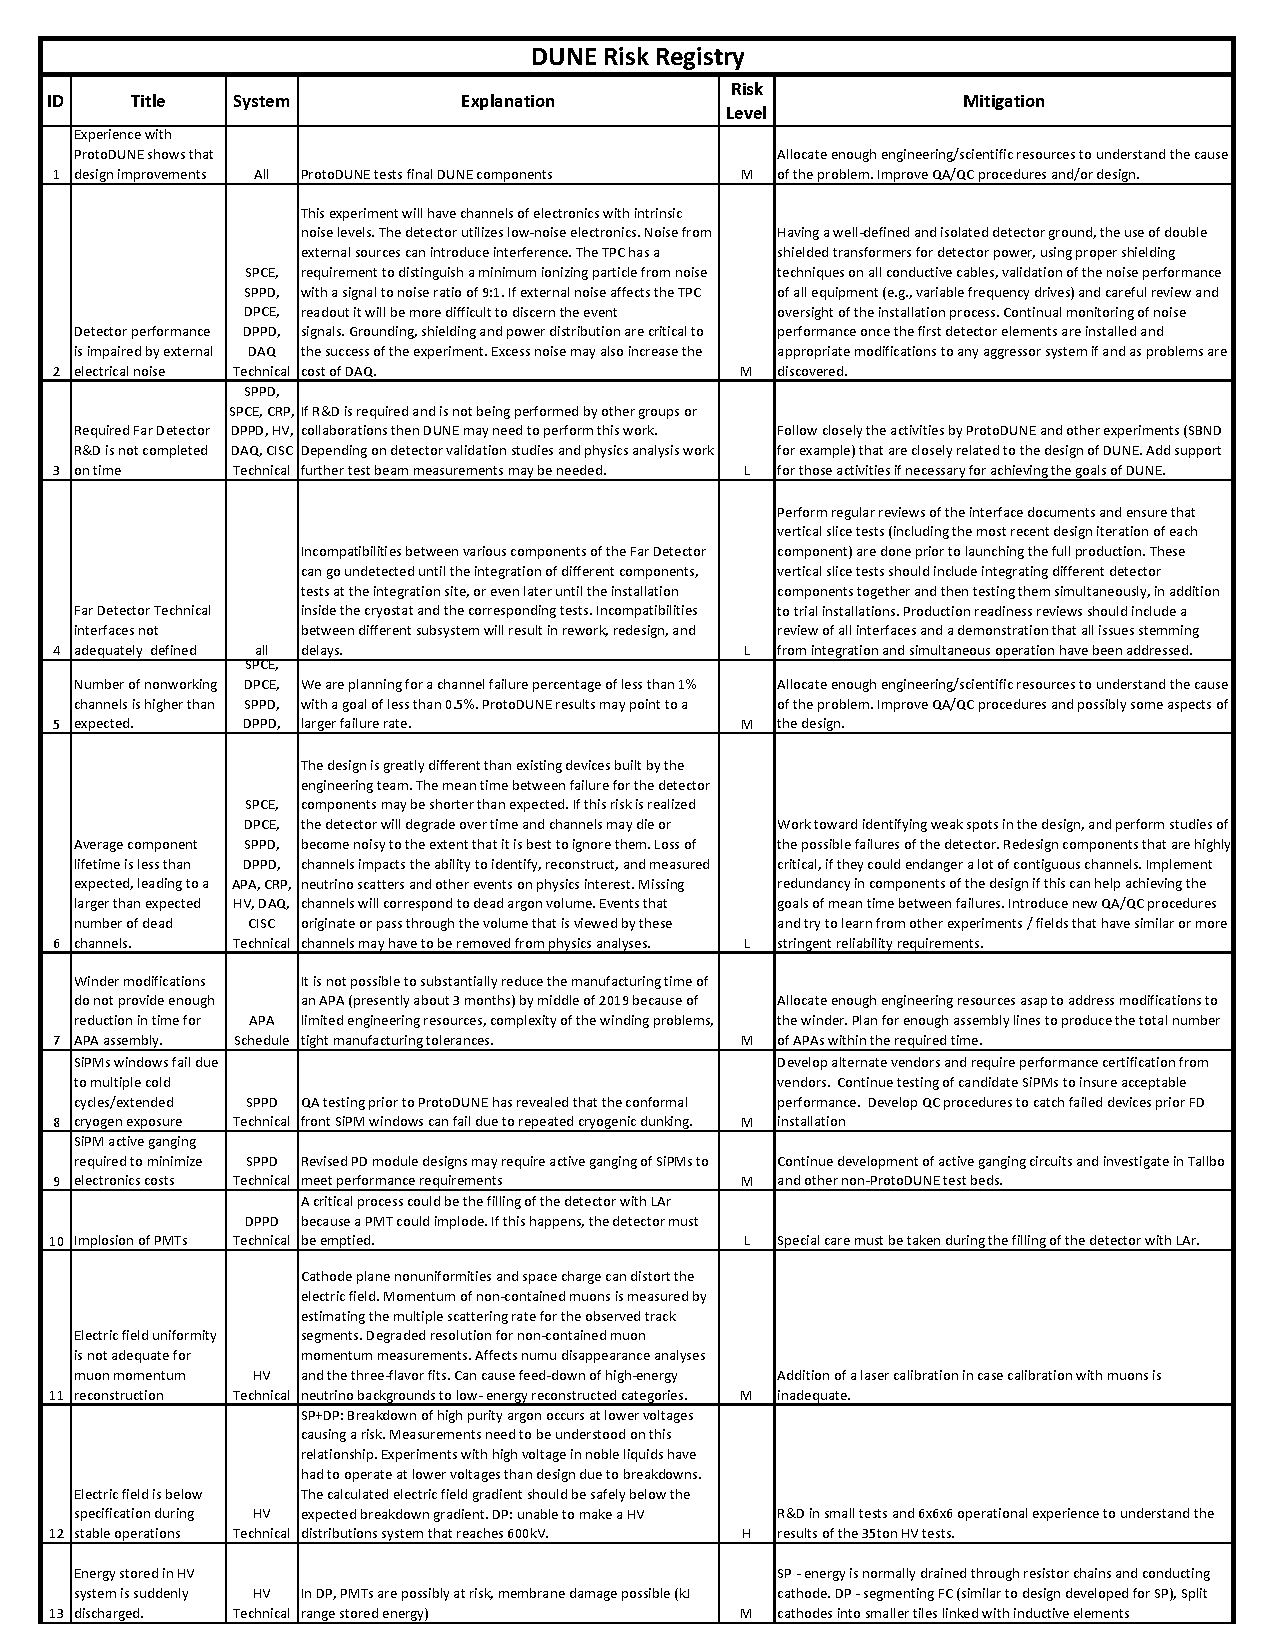
\includegraphics[width=0.99\textwidth]{DUNE_Risks_v4b1}
\end{dunefigure}
\begin{dunefigure}[\dword{dune} overall risk register]{fig:dune_risks2}
  {Second page of \dword{dune} overall risk register.}
  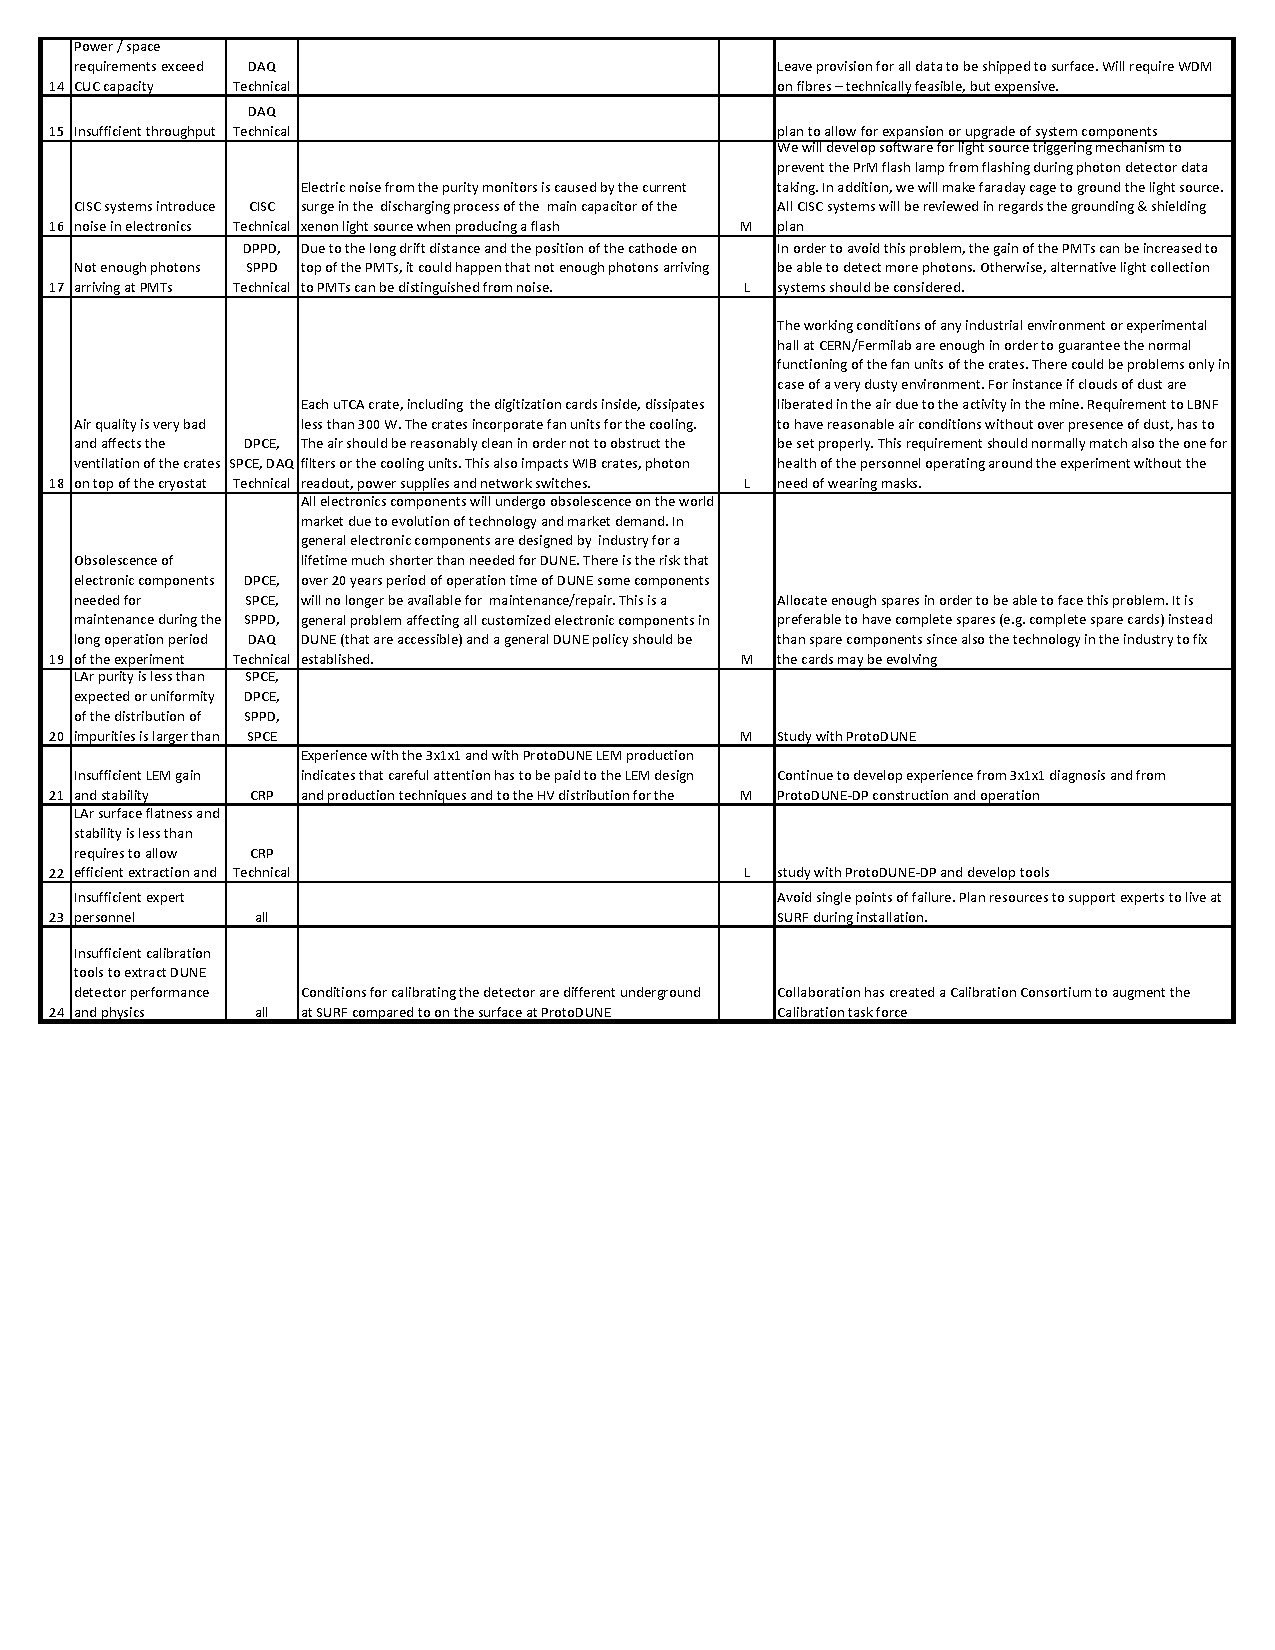
\includegraphics[width=\textwidth]{DUNE_Risks_v4b2}
\end{dunefigure}
\dword{lbnf} and \dword{dune}-US would like \dword{dune} to update and
expand this risk register to allow a Monte Carlo analysis of cost and
schedule risks to the \dword{us} project resulting from international
\dword{dune} risks. This request is under consideration.

One update to the risk registry has been for \dword{tc}, in which some
risks  associated with  DUNE  integration and  installation have  been
added. Table~\ref{fig:tc_risks} summarizes the \dword{tc} risks.
\begin{dunefigure}[\dword{tc} risks]{fig:tc_risks}
  {\dword{tc} risk register.}
  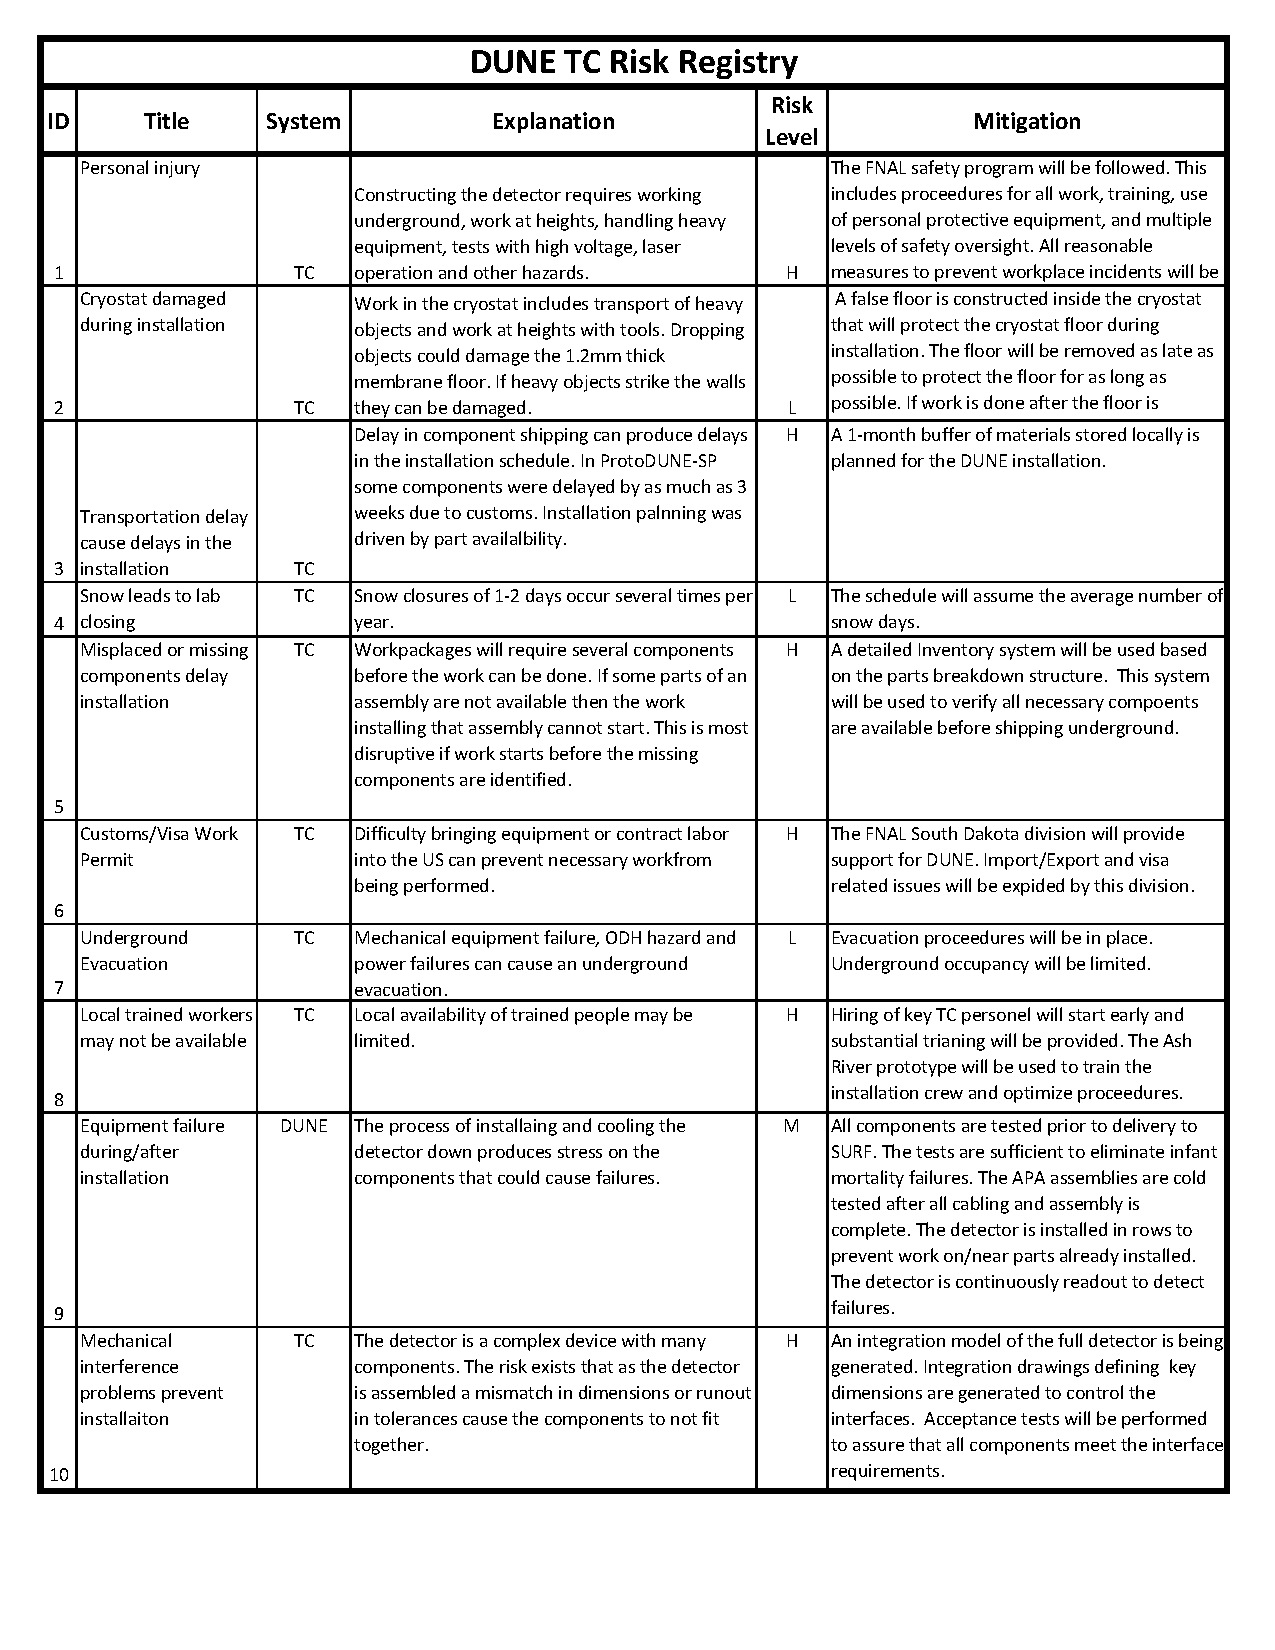
\includegraphics[width=\textwidth]{TC_Risks_v4b}
\end{dunefigure}

The next update of the risk register will separate the current overall
risk level into separate quantified probability and impact.

Successfully operating \dword{protodune} retires many
potential risks in \dword{dune} itself. This includes most risks associated with the
technical design, production processes, \dword{qa}, integration
and installation. Residual risks remain relating to design and
production modifications associated with scaling to \dword{dune}, mitigations
to known installation and performance issues in \dword{protodune}, underground
installation at \surf and organizational growth.

The highest technical risks include development of a system to
deliver \SI{600}{kV} to the \dual cathode; general delivery of the
required \dword{hv}; cathode and \dword{fc} discharge to the cryostat
membrane; noise levels, particularly for the \dword{ce}; %cold TPC electronics,
number of dead channels; lifetime of components surpassing \dunelifetime{}; %20 years,
\dword{qc} of all components; verification of improved \dword{lem}
performance; verification of new cold  \dword{adc} and  \dword{coldata} performance;
argon purity; electron drift lifetime; \phel light yield;
incomplete calibration plan; and incomplete connection of design to
physics. Other major risks include insufficient funding, optimistic
production schedules, incomplete plans for integration, testing and installation.

Key risks for \dword{tc} to manage include the following:
\begin{enumerate}
\item Consortia leave too much scope unaccounted for and too much falls
  to  the \dword{comfund}.
\item Insufficient organizational systems are put into place to
  ensure that this complex international mega-science project,
  including \dword{tc}, \fnal as host laboratory, \surf, DOE, and all international
  partners continue to work together successfully to ensure
  appropriate processes and services are provided for the success of
  the project.
\item Inability of \dword{tc} to obtain sufficient personnel resources to
  ensure that \dword{tc} can oversee and coordinate all project tasks.  While the \dword{us}, 
  as host country, has a special responsibility to \dword{tc}, personnel resources should
  be directed to \dword{tc} from each collaborating country. 
\end{enumerate}

The consortia have provided preliminary versions of risk analyses that
have been collected on the \dword{tc} webpage (DocDB-6443). These have
been developed into an overall risk register that will be monitored
and maintained by \dword{tc} in coordination with the consortia.  The
next update of the risk register is planned for spring 2019, in
advance of the final \dword{tdr} submission.

%%%%%%%%%%%%%%%%%%%%%%%%%%%%%%%%
\section{Requirements}
\label{sec:fdsp-coord-requirements}

The scientific goals of \dword{dune} as described in \dword{dune}
\dword{tdr} Volume~\volnumberexec:~\voltitleexec include
\begin{itemize}
\item a comprehensive program of neutrino oscillation measurements
  including the search for CP violation
\item measurement of $\nu_{e}$ flux from a core-collapse supernova within our
  galaxy should one occur during \dword{dune} operations
\item searching for baryon number violation
\end{itemize}
These goals motivate a number of key detector requirements: drift
field, electron lifetime, system noise, photon detector light yield
and time resolution. The \dword{exb} has approved a list of high
level detector specifications, including those listed above. These are
maintained in edms-xxxx, and the high level requirements with
significant impact on physics are highlighted in
Table~\ref{tab:dunephysicsreqs}.
\begin{dunetable}
  [\dword{dune} physics-related specifications owned by \dword{exb}]
  {p{0.025\textwidth}p{0.06\textwidth}p{0.2\textwidth}p{0.35\textwidth}p{0.15\textwidth}p{0.1\textwidth}}
  {tab:dunephysicsreqs}
  {\dword{dune} physics-related specifications owned by \dword{exb}}
  ID & System & Parameter & Physics Requirement Driver & Requirement & Goal \\ \toprowrule
  1   & HVS    & Minimum drift field &  Limit recombination, diffusion and space charge impacts on particle ID. Establish adequate \dword{s/n} for tracking. & >\SI{250}{V/cm} & \spmaxfield \\ \colhline
  2   & CE     & System noise & The noise specification is driven by pattern recognition and two-track separation.  & <\SI{1000}{enc} & ALARA \\ \colhline
  3   & PDS    & Light yield  & The light yield shall be sufficient to measure time of events with visible energy above 200 MeV.  Goal is 10\% energy measurement for visible energy of 10 MeV.  & >\SI{0.5}{pe/MeV} & >\SI{5}{pe/MeV}  \\ \colhline
  4   & PDS    & Time resolution  & The time resolution of the photon detection system shall be sufficient to assign a unique event time.  & $<\,\SI{1}{\micro\second}$ & $<\,\SI{100}{\nano\second}$  \\ \colhline
  5   & all    & liquid argon purity & The LAr purity shall be sufficient to enable drift e- lifetime of 3 (10)ms & $<$\,\SI{100}{ppt} & $<$\,\SI{30}{ppt} \\ \colhline
\end{dunetable}
Eleven other significant specifications owned by the \dword{exb} are
listed in Table~\ref{tab:dunephysicsspecs} along with another twelve
high level engineering specifications.
\begin{dunetable}
  [\dword{dune} physics-related specifications owned by \dword{exb}]
  {p{0.025\textwidth}p{0.06\textwidth}p{0.2\textwidth}p{0.35\textwidth}p{0.15\textwidth}p{0.1\textwidth}}
  {tab:dunephysicsspecs}
  {\dword{dune} high level system specifications owned by \dword{exb}}
  ID & System & Parameter & Physics Requirement Driver & Requirement & Goal \\ \toprowrule
  6   & APA & Gaps between APAs  & minimize events lost due to vertex in gaps between APAs (15mm on same support beam, 30mm on adjacent beams) & <\SI{30}{mm} & <\SI{15}{mm} \\ \colhline
  7   & DSS & Drift field uniformity & tolerance on drift field due to component location & $<\,\SI{1}{\%}$  &   \\ \colhline
  8   & APA & wire angles  & 0$^\circ$ collection, $\pm$35.7$^\circ$ induction &  &  \\ \colhline
  9   & APA & wire spacing  & \SI{4.669}{mm} for U,V; \SI{4.790}{mm} for X,G &  &  \\ \colhline
  10  & APA & wire position tolerance  & & $\pm\,\SI{0.5}{mm}$  &  \\ \colhline
  11  & HVS & Drift field uniformity & tolerance on drift field due to HVS system & $<\,\SI{1}{\%}$  &  \\ \colhline
  12  & HVS & Cathode power supply ripple & very small compared to intrinsic electronics noise & $<\,\SI{100}{enc}$ &   \\ \colhline
  13  & CE & Frontend peaking time  & optimize vertex resolution & \SI{1}{\micro\second} &  \\ \colhline
  14  & CE & Signal saturation  & largest signals occur with multiple protons in the primary vertex & 500k $e^-$ &  \\ \colhline
  15  & cryo & LAr N$_2$ contamination  & optical attenuation length in liquid argon with 50~ppm of N$_2$ contamination is roughly 3~m & $<\,\SI{25}{ppm}$ &  \\ \colhline
  16  & all & Detector dead time  & risk of missing a supernova burst if all operating cryostats are offline & $<\,\SI{0.5}{\%}$ &  \\ \colhline
\end{dunetable}
The high level \dword{dune} requirements that drive the \dword{lbnf} design are
maintained in DocDB-112 and under change control. These are owned by
the \dword{dune} \dword{tc} and the \dword{lbnf} project manager.

Lower level detector specifications are held by the consortia and
described in the \dword{dune} \dword{tdr} \dword{dsp}
Volume~\volnumbersp\ and \dword{ddp} Volume~\volnumberdp\ chapters for
each consortium. A complete list of detector specifications is
provided in Chapter~\ref{ch:tc-sp-reqs}.


%%%%%%%%%%%%%%%%%%%%%%%%%%%%%%%%
\section{Value Engineering}
\label{sec:fdsp-coord-ve}

Value engineering is the ongoing process of arriving at cost effective
solutions to the technical challenges of building the \dword{dune}
detector. \dword{dune} value engineering builds on significant
developments in \dword{lar} detectors dating to the early 1970s,
especially the large \dwords{lartpc}: ICARUS and
\dword{microboone}. Prototyping by both LBNE and LBNO has
significantly advanced the value engineering process, leading to
construction of the \dword{protodune} detectors. These detectors validate
\dword{dune} designs and confirm that the necessary performance is
met. Any significant departure from current designs must account for
the success of \dword{protodune} and may require testing in a second
run of \dword{protodune}. The value engineering process is executed at
both the consortia and \dword{tc} level.

For example, the \dword{apa} size has been optimized over the last 10--15 years,
using input from dimensions of the Ross shaft, shipping container size
and availability of hih quality long stainless steel tubes from reliable vendors.
At this point, any significant change to the \dword{apa} design would likely
lead to new and significant re-engineering costs.

\fixme{Do we want to describe highlights of all of the VE that has been done
over the last 10 years? Do we want to discuss possible scope options/reductions?}

%%%%%%%%%%%%%%%%%%%%%%%%%%%%%%%%
\section{Lessons Learned}
\label{sec:fdsp-coord-lessons}

A detailed list of lessons learned from construction and operation of
\dword{pdsp} is in DocDB-8255. These lessons have driven planning for
\dword{dune} and have led to some design changes in
\dword{dune}. Lessons learned will continue to be updated throughout
the final design stage and into production. The methodologies are
described in Section~\ref{sec:lessons_learned}.

%%%%%%%%%%%%%%%%%%%%%%%%%%%%%%%%
\section{Interface to National Projects}
\label{sec:fdsp-coord-national}

\dword{dune} \dword{tc} works with each consortium leadership team. The
consortia leadership teams comprise the consortia leaders and 
consortia technical leaders as well as others appointed by the consortia
leaders. The consortia leadership teams usually have representatives
from the various national projects that provide the funding to build the consortia
deliverables. If the consortia leadership teams are not directly
embedded in the various national projects building their subsystem,
then the consortia leadership teams must still represent their national projects
to \dword{tc}. The consortia leadership teams are responsible for
providing their deliverables on time according to the
\dword{ims}. They are responsible for identifying any inconsistencies
between the \dword{ims} and their national project schedules and
bringing these issues to \dword{tc}. The consortia leadership teams
are responsible for reporting progress against the \dword{ims} to
\dword{tc}.

%%%%%%%%%%%%%%%%%%%%%%%%%%%%%%%%
\section{Reporting}
\label{sec:fdsp-coord-reporting}

The \dword{dune} project has published regular monthly reports since
the final design and construction of \dword{protodune} began in
earnest in summer 2016. \Dword{tc} will continue to compile and publish these
reports. Reporting will expand to include monthly reports against the
\dword{ims}. The \dword{dune} project provides regular reports to the
LBNC at reviews several times a year. The \dword{dune} project
produces reports from design, production and operations reviews.

%%%%%%%%%%%%%%%%%%%%%%%%%%%%%%%%
%\section{Management of Schedule and Risks}
%\label{sec:fdsp-coord-mgmt}


%%%%%%%%%%%%%%%%%%%%%%%%%%%%%%%%
%\section{Design Process}
%\label{sec:fdsp-coord-designprocess}

%The design process follows the engineering safety process and review
%processes described in Chapter~\ref{vl:tc-review}. The current status
%of defining international code equivalences is described in
%Section~\ref{sec:esh_codes}.

%%%%%%%%%%%%%%%%%%%%%%%%%%%%%%%%
%\section{Integration Facility}
%\label{sec:fdsp-coord-itf}
%
%Do we explain the concept of ITF here in general terms? May be better
%in Chapter~\ref{vl:tc-facility}?
